% Anexo · Bitácora de supuestos. Cifras verificadas contra output/cifras.md.

\section*{Anexo. Bitácora de supuestos}
\addcontentsline{toc}{section}{Anexo. Bitácora de supuestos}

Origen de cada hallazgo: \textbf{(V)} verbalizado por la contraparte, \textbf{(M)} medido sobre los datos, \textbf{(I)} inferido por el equipo. Las consultas enviadas por el hilo de correo no fueron respondidas, de modo que los supuestos quedan cerrados con criterio propio y cuantificados.

\begin{longtable}{p{0.6cm} p{3.0cm} c p{4.3cm} p{4.3cm} p{2.0cm}}
\toprule
\textbf{ID} & \textbf{Supuesto} & \textbf{Origen} & \textbf{Justificación} & \textbf{Efecto si fuera falso} & \textbf{Decisión} \\
\midrule
\endhead

\textbf{S1} & Una caja rinde 9,0\,L en los dos formatos (12$\times$750\,ml y 6$\times$1500\,ml). & M/I & El maestro de costos lo declara para ambos (M) y la aritmética de los formatos da 9\,L exactos. El precio de lista por caja coincide entre magnum y gran reserva estándar (77,26 y 77,20 USD) y el costo por caja es idéntico (M), lo que solo se sostiene si rinden lo mismo (I). & Con 18\,L el precio medio anual sería 4,47 USD/L ($-$7,5\,\%); con 4,5\,L, 5,03 (+4,2\,\%). La mezcla sigue explicando 108\,\% del alza en los tres casos: la conclusión no cambia. & Equipo, 4 sep \\
\midrule
\textbf{S2} & Las cajas cargadas como botellas se dividen por 12 o por 10. & M & 151 líneas cuyo total no cuadra con el embarque de la misma venta; el factor se identifica contra \texttt{origen\_embarques.json} (M). & Sin corregir, los litros se sobreestiman y el precio por litro baja artificialmente en esas líneas. & Equipo, sep \\
\midrule
\textbf{S3} & El monto neto se recalcula como cajas $\times$ precio $\times$ (1 $-$ descuento) cuando el registrado difiere más de 0,5\,\%. & V/M & El 94,5\,\% de las filas cuadra con esa fórmula a $\pm$0,5\,\% (M), así que la fórmula es la regla y el resto es ruido de carga. La gerencia declaró que «en esta empresa no se pierde ni un peso» (V). & Si el monto registrado fuera el real (por ejemplo, rebates no declarados), el ingreso de exportación cambiaría en CLP 2.096 millones. & Equipo, sep \\
\midrule
\textbf{S4} & La moneda vacía se imputa por mercado: Chile en CLP, el resto en USD. & M & 698 registros sin moneda (5,0\,\%), repartidos de forma pareja por mercado, vendedor, mes y cliente: no hay patrón de negocio, es pérdida de campo en la carga (M). Los rangos de precio separan ambas monedas sin ambigüedad (20.428--72.290 en CLP, 22--80 en USD). & Filas convertidas con la moneda equivocada: error de escala de tres órdenes de magnitud. & Equipo, sep \\
\midrule
\textbf{S5} & Los costos ausentes se imputan por tier y añada. & M & Las 81 filas del maestro siguen una regla determinista por tier y añada, sin una sola excepción (M). Faltan 15 pares de la añada 2021 y un valor \texttt{N/A}. & No afecta el precio por litro ni la facturación; cambiaría el margen bruto en el 17,4\,\% de las filas del universo. & Equipo, sep \\
\midrule
\textbf{S6} & Los montos se convierten a pesos con el dólar observado de la fecha de factura. & V/I & Finanzas no tiene política formal de tipo de cambio (V), pero sí declaró que el año «se cierra por factura, no por despacho» (V); adoptamos la misma fecha por consistencia (I). & El ingreso en pesos varía $-$0,91\,\% a fecha de embarque y $-$2,14\,\% a fecha de cobranza (60 días hemisferio sur, 90 norte). No afecta la métrica, que está en USD/L. & Contraparte (cierre) y equipo (conversión), 4 sep \\
\midrule
\textbf{S7} & Las líneas negativas son merma: restan litros e ingreso, pero su costo no se reversa. & V/I & «Si se pierde la cadena de frío se descartan esas cajas; es considerado dentro de la merma» (V). El vino se produjo y se perdió, así que el costo ya se devengó (I). & Reversar el costo subiría el margen bruto de 47,25\,\% a 48,05\,\%, una diferencia de CLP 419 millones. & Contraparte y equipo, 4 sep \\
\midrule
\textbf{S8} & La comparación entre semestres mide un cambio de mezcla estructural y no solo estacionalidad. & M/I & Es el supuesto más expuesto, porque solo hay un año de datos y la contraparte declaró que la venta es contracíclica al hemisferio norte con «fuerte estacionalidad en el cambio de estación» (V). Tres mediciones apuntan en contra de esa explicación (M): \textbf{(a)} Brasil, el único mercado de exportación del hemisferio sur, sube de 22,7\,\% a 31,5\,\% de gran reserva, igual que los del norte; una estacionalidad de fin de año del hemisferio norte no debería aparecer ahí. \textbf{(b)} La participación mensual sube de forma sostenida, de 19,8\,\% en enero a 35,9\,\% en noviembre, y diciembre baja a 35,2\,\%: no tiene forma de peak de temporada. \textbf{(c)} Los diez mercados suben entre 7,5 y 12,3 pp, así que no es un cliente ni una región. & Con un año no se puede descartar del todo un componente estacional (I). Si el alza fuera puramente cíclica, la premiumización se revertiría en el 1.\textsuperscript{er} semestre de 2026 y la recomendación pasaría de dirigir la mezcla a planificar stock estacional. La magnitud del efecto en 2025 (CLP 2.961 millones) no cambia. & Equipo, oct \\
\midrule
\textbf{S9} & La mezcla se descompone a nivel de tier (tres categorías). & V/I & Es el nivel que la contraparte nombró como el que no disgrega al decidir (V) y el que separa los precios por litro sin solapamiento: 2,5, 4,7 y 8,3 USD/L (M). & Descomponer por los 24 productos reparte el efecto en más celdas, pero no cambia el signo ni el orden de magnitud de la mezcla. & Equipo, sep \\
\midrule
\textbf{S10} & El dólar observado representa el tipo de cambio efectivamente liquidado. & I & La contraparte no mencionó cobertura cambiaria en toda la reunión, ni al preguntarle por el tipo de cambio (V); asumimos que no la hay (I). & Con forwards, el ingreso en pesos sería distinto del que calculamos. No afecta la métrica en USD/L ni la descomposición. & Equipo, sep \\
\midrule
\textbf{S11} & El tramo cambiario dólar-euro queda fuera del modelo. & V/M & «Todos los contratos se hacen en dólares, pero los clientes europeos pagan en euros» (V). No hay paridad USD/EUR en ninguna de las cuatro fuentes (M). & Afecta al 32\,\% del ingreso de exportación (Alemania, Países Bajos y Reino Unido) al convertir a pesos, pero no el valor facturado en dólares. & Contraparte y equipo, 4 sep \\
\midrule
\textbf{S12} & Las fechas ambiguas \texttt{dd/mm/aaaa} se leen como día/mes. & M & Es el formato declarado de los otros tres patrones de fecha del mismo campo (M). La columna \texttt{mes} del ERP no sirve para dirimirlo: discrepa de la fecha en 981 filas, también en fechas ISO sin ambigüedad (M). & 1.387 fechas admiten las dos lecturas; 121 de ellas calzarían con la columna \texttt{mes} leídas como mes/día. Leerlas al revés movería de mes a lo más esas 121 líneas, sin efecto en la agregación semestral salvo las que cruzan junio o diciembre. & Equipo, sep \\
\midrule
\textbf{S13} & El mercado de Corea del Sur, con \texttt{zona\_id} 8 inexistente, se asigna a Asia. & I & La tabla de zonas llega hasta 5 y los demás mercados asiáticos están en Asia (M). & Sin corregir, 1.059 líneas quedan sin zona y Asia queda subrepresentada en los cortes por región. & Equipo, sep \\
\bottomrule
\end{longtable}

\begin{figure}[!htbp]
  \centering
  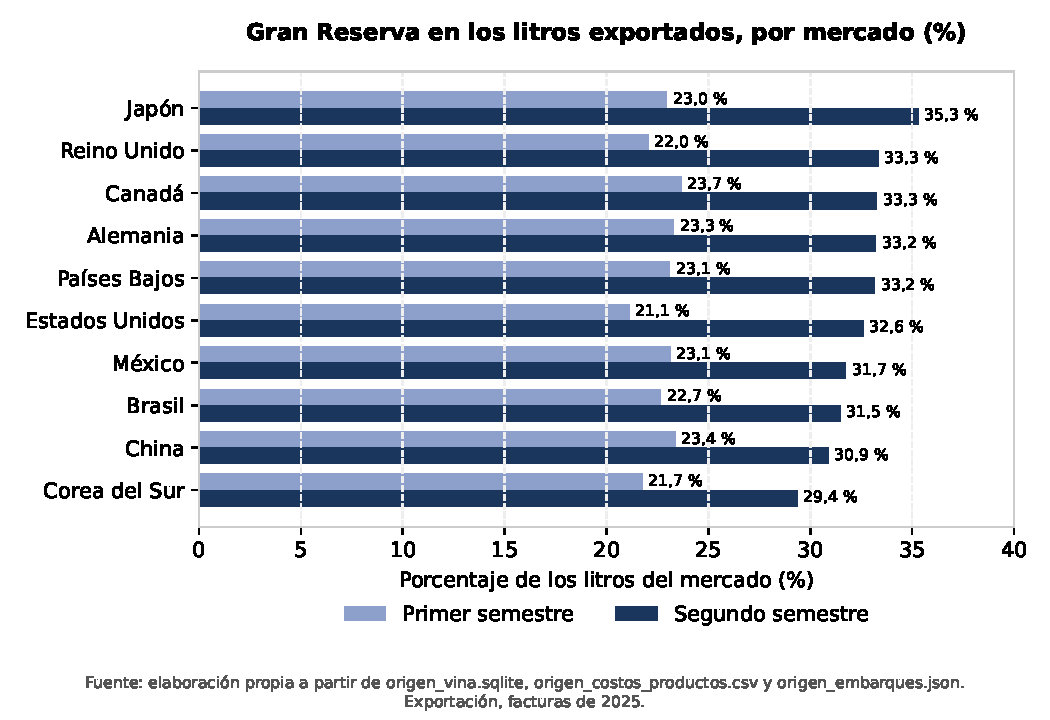
\includegraphics[width=0.58\linewidth]{figura4_gran_reserva_mercados.pdf}
  \caption{Participación de gran reserva en los litros, por mercado y semestre, \%. Fuente: elaboración propia sobre \texttt{fact\_venta}.}
  \label{fig:mercados}
\end{figure}

\noindent La figura respalda el supuesto S8: los diez mercados de exportación suben su participación de gran reserva entre el 1.\textsuperscript{er} y el 2.\textsuperscript{o} semestre, entre 7,5 pp (China) y 12,3 pp (Japón). Brasil, el único del hemisferio sur, sube 8,8 pp.
